\documentclass{beamer}
\usetheme{Warsaw}

\usepackage[utf8]{inputenc}
\usepackage{fancybox}
\usepackage{multimedia} 
\usepackage{subfig}
\usepackage{amsmath}
\usepackage{hyperref}
\usepackage[all]{xy}
\begin{document}


\title[Angewandte Mathematik] % (optional, only for long titles)
{Angewandte Mathematik
\\

\includegraphics[scale=0.15]{images/cover}
}
\subtitle{}
\author[Dr. Johannes Riesterer] % (optional, for multiple authors)
{Dr.  rer. nat. Johannes Riesterer}

\date[KPT 2004] % (optional)
{}

\subject{Angewandte Mathematik}

\frame{\titlepage}

\begin{frame}
    \frametitle{Angewandte Mathematik}
\framesubtitle{}
    \begin{block}{Kann jeder Mathematik lernen?}
\begin{itemize}
\pause \item Mathematik hat ein Motivationsproblem
\pause \item Jeder kann Mathematik lernen, aber Mathematik unterrichten ist sehr schwer, da jeder individuelle Materialien braucht.
\pause \item Eigeninitiative ist nötig

\end{itemize}
\end{block}

 \end{frame}


\begin{frame}
    \frametitle{Angewandte Mathematik}
\framesubtitle{}
    \begin{block}{Konstruktivismus}
 Der mathematische Konstruktivismus ist eine Richtung der Philosophie der Mathematik, die den ontologischen Standpunkt vertritt, dass die Existenz mathematischer Objekte durch ihre Konstruktion zu begründen ist. 
\end{block}
    \begin{block}{Platonismus}
Mathematische Gegenstände (Zahlen, geometrische Figuren, Strukturen) und Gesetze sind keine Konzepte, die im Kopf des Mathematikers entstehen, sondern es wird ihnen eine vom menschlichen Denken unabhängige Existenz zugesprochen.
\end{block}
 \end{frame}


\begin{frame}
    \frametitle{Angewandte Mathematik}
\framesubtitle{}
    \begin{block}{Was ist (angewandte) Mathematik?}
\begin{itemize}
\pause \item Algorithmen zum Lösen von Problemen.
\pause \item Abschätzungen, wie gut und genau die Algorithmen funktionieren.
\pause \item Mathematische Grundlagen, auf denen Algorithmen und Abschätzungen basieren. 
\pause \item Softwaretechnische Aspekte in Bezug auf  Implementierung der Algorithmen.
\end{itemize}
\end{block}
 \end{frame}

\begin{frame}
    \frametitle{Angewandte Mathematik}
\framesubtitle{}
    \begin{block}{Mathematische Modellierung}
\begin{figure}[H]
      \centering
    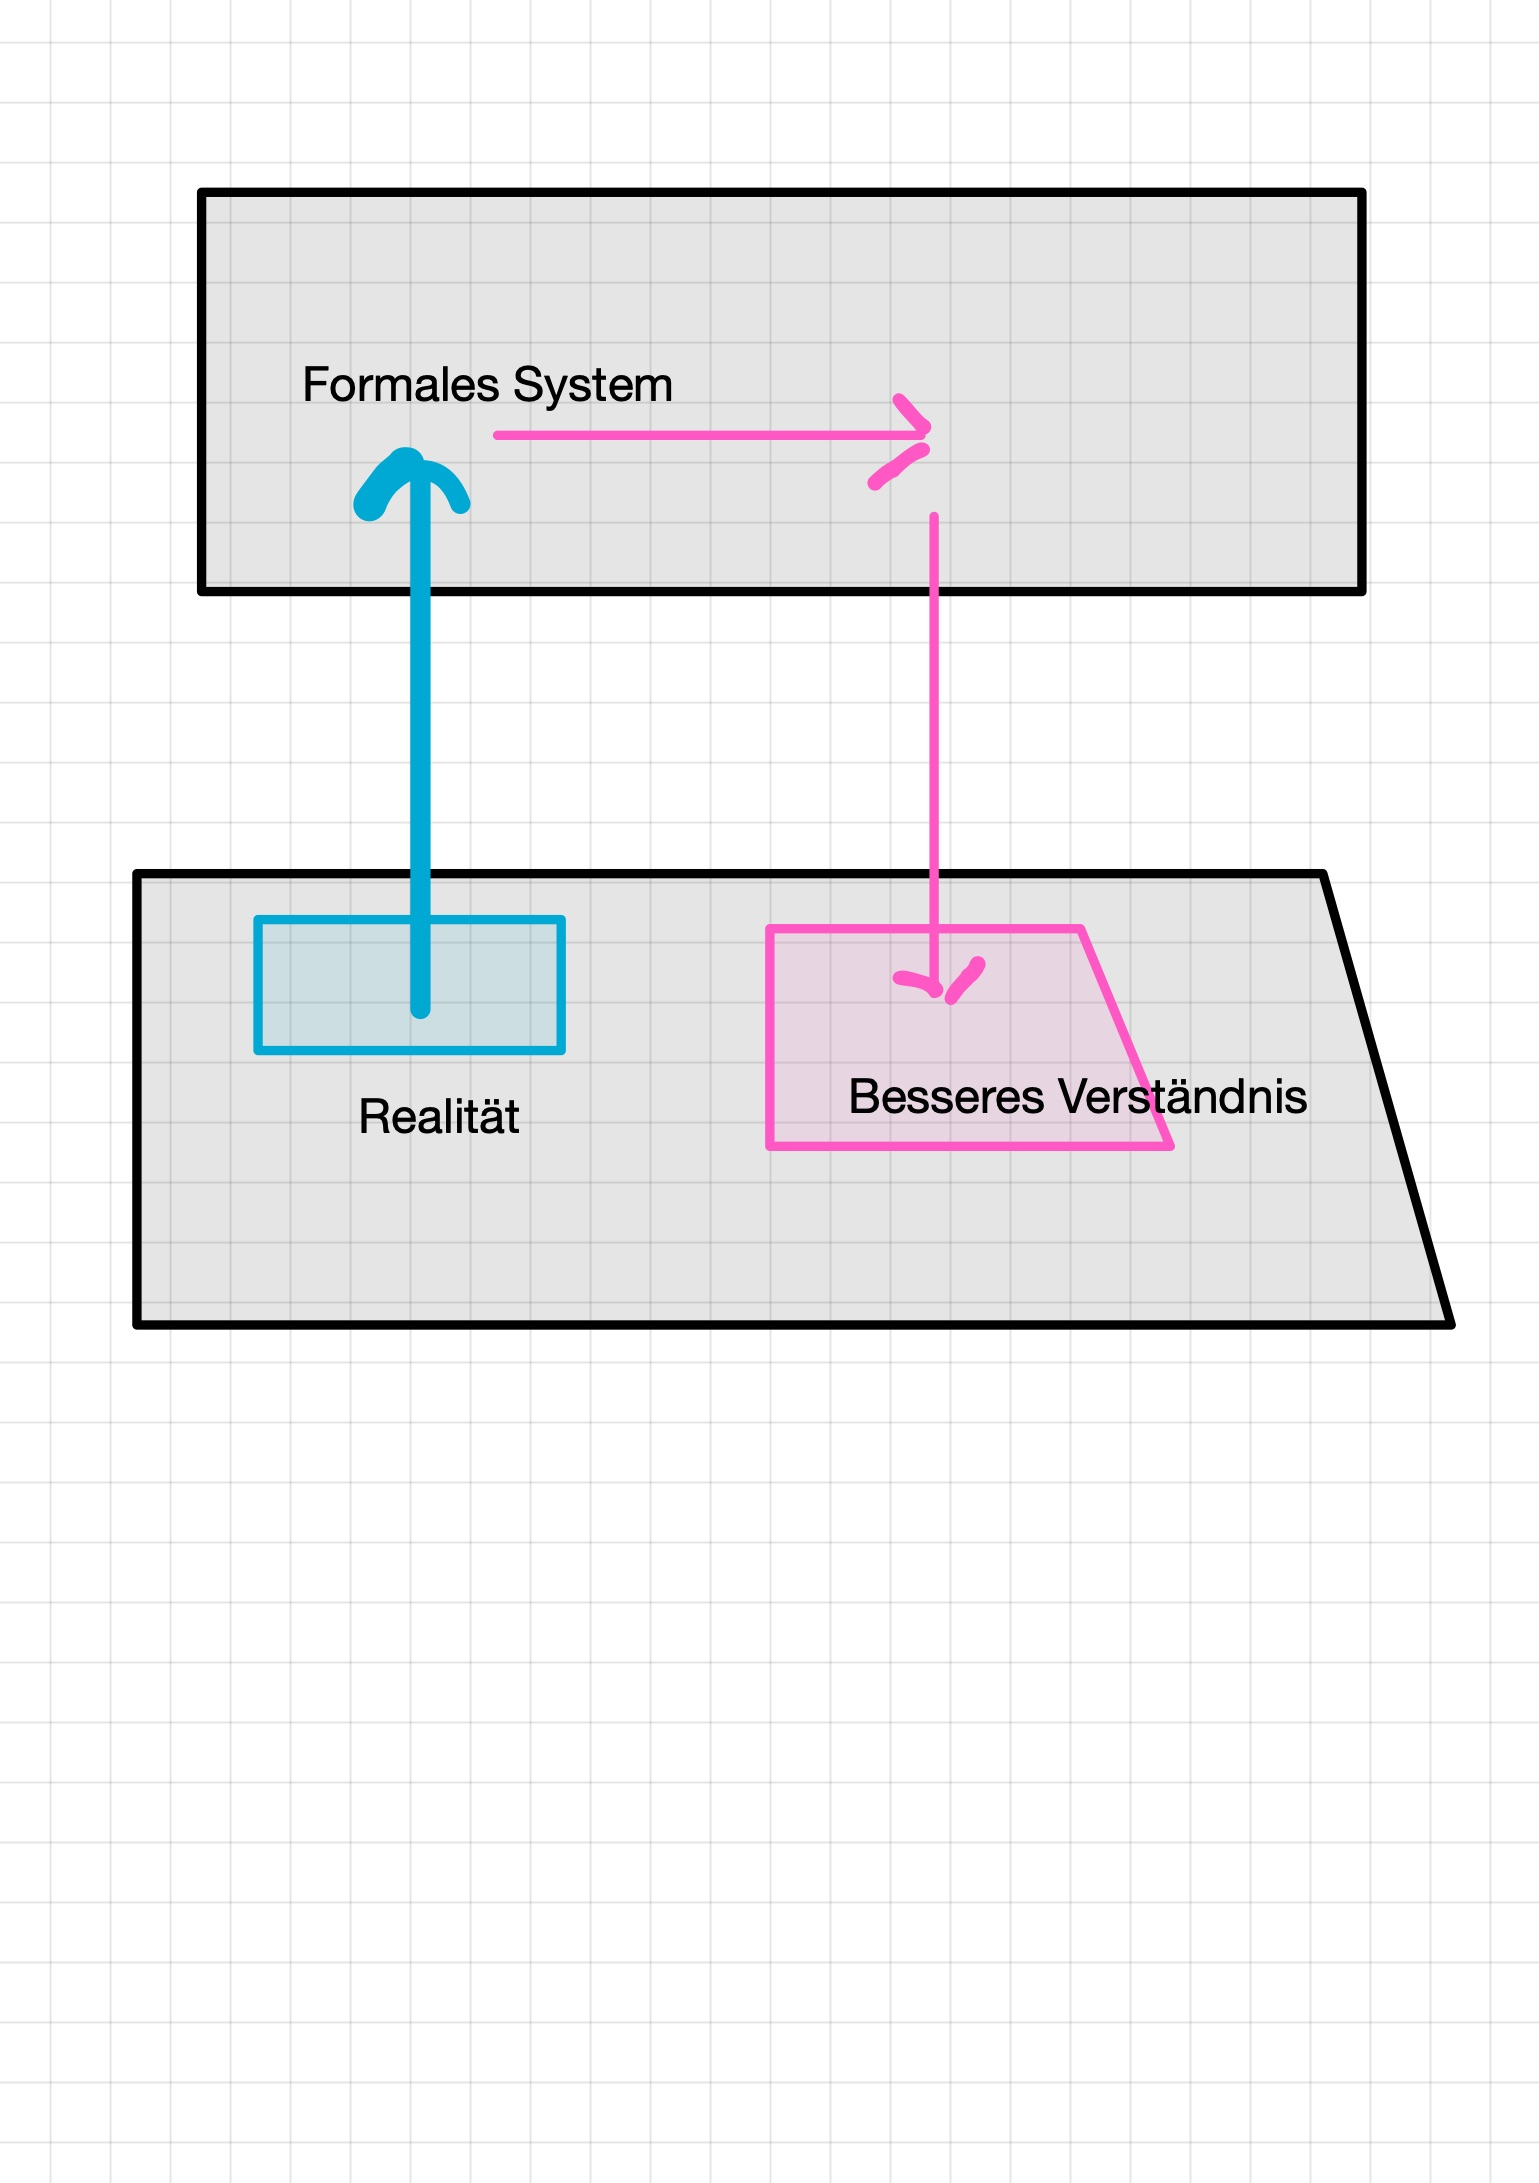
\includegraphics[width=0.7\textwidth]{images/modellierung}
      \caption{Quelle: Wikipedia: }
\end{figure}
\end{block}
 \end{frame}


\begin{frame}
\framesubtitle{Algorithmus}
    \begin{block}{Algorithmus}
\begin{figure}[H]
      \centering
    
\includegraphics[width=0.7\textwidth]{images/algo}
      \caption{Quelle: Wikipedia}
\end{figure}
\end{block}

 \end{frame}




\begin{frame}
    \frametitle{Angewandte Mathematik}
\framesubtitle{}
    \begin{block}{Algorithmus Informell}
Ein Algorithmus ist eine eindeutige Handlungsvorschrift zur Lösung eines Problems oder einer Klasse von Problemen. Algorithmen bestehen aus endlich vielen, wohldefinierten Einzelschritten.
\end{block}
    \begin{block}{Algorithmus Formal}
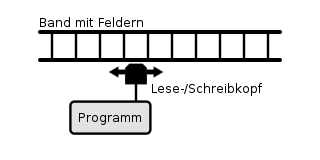
\includegraphics[scale=0.8]{images/Turingmaschine}
\end{block}
 \end{frame}


\begin{frame}
\framesubtitle{Limes}
    \begin{block}{Achilles und die Schildkröte}
\begin{figure}[H]
      \centering
    
\includegraphics[width=0.7\textwidth]{images/archilles}
      \caption{Quelle: https://physics.mit.edu/news/provoked-by-zenos-paradoxes/}
\end{figure}
\end{block}

 \end{frame}


\begin{frame}
    \frametitle{Angewandte Mathematik}
\framesubtitle{Limes}
    \begin{block}{Achilles und die Schildkröte}
\begin{figure}[H]
      \centering
    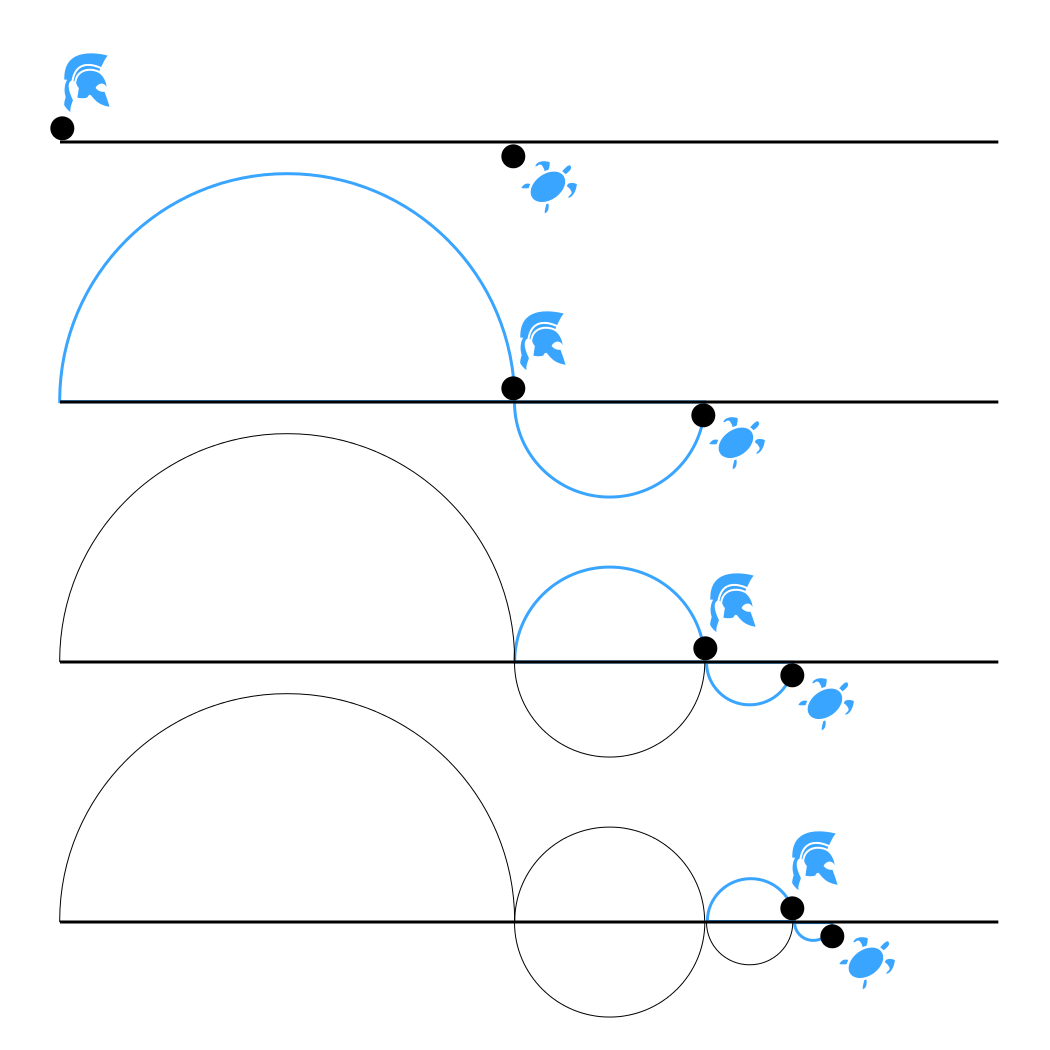
\includegraphics[width=0.3\textwidth]{images/Zeno_Achilles_Paradox}
      \caption{Quelle: Wikipedia: }
\end{figure}
\href{https://www.youtube.com/watch?v=X8Qksx_Ng9k}{Mehr hier im Video}
\end{block}
  \begin{block}{Paradoxon der Antike}
 Obwohl Achilles schneller ist, kann er die Schildkröte niemals einholen.
\end{block}
 \end{frame}


\begin{frame}
    \frametitle{Angewandte Mathematik}
\framesubtitle{Limes}
    \begin{block}{Achilles und die Schildkröte infinitessimal betrachtet}
Sei $s_0$ der Vorsprung der Schildkröte zu Beginn des Rennens, $t_0$ die Zeit, die Achilles benötigt, um $s_0$ zurückzulegen. Die Schildkröte ist $q$-mal langsamer als Achilles.
Dann holt Achilles die Schildkröte nach der Zeit $t_0 \cdot q$ ein weiteres Mal ein, nach der Zeit $(t_0 \cdot q) \cdot q = t_0 \cdot q^2$ ein drittes Mal usw.
Mit $q^0 = 1$ ist die Summe aller betrachteten Zeiten, die Achilles zurücklegt:

$t = t_0 \cdot \sum_{n=0}^\infty q^n = t_0 \cdot \lim_{n \to \infty} \sum_{k=0}^{n} q^{k} = t_0 \cdot \lim_{n \to \infty} \frac{1 - q^{n+1}}{1 -q} = \frac{t_0}{1 -q}$.
\end{block}
 \end{frame}




\begin{frame}
    \frametitle{Mehrdimensionale Differentialrechnung}
\framesubtitle{Limes}
    \begin{block}{Konvergenz}
\begin{figure}[H]
      \centering
    
\includegraphics[width=0.6\textwidth]{images/newton}
      \caption{Quelle: DALLE}
\end{figure}

\end{block}

 \end{frame}


\begin{frame}
    \frametitle{Mehrdimensionale Differentialrechnung}
\framesubtitle{Limes}
    \begin{block}{Konvergenz}
\begin{figure}[H]
      \centering
    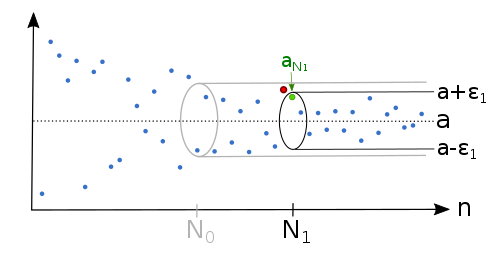
\includegraphics[width=0.8\textwidth]{images/500px-Epsilonschlauch_klein}
      \caption{Quelle: Wikipedia: https://commons.wikimedia.org/wiki/File:Epsilonschlauch\_klein.svg}
\end{figure}

\end{block}

 \end{frame}






\begin{frame}
    \frametitle{Mehrdimensionale Differentialrechnung}
\framesubtitle{Limes}
    \begin{block}{Konvergenz}
Eine Folge $(a_n)$ in $\mathbb{R}^n$ heißt konvergent gegen den Grenzwert $a \in \mathbb{R}^n$, wenn gilt:
\begin{align*}
\forall {\varepsilon > 0} \ \exists \ N \in \mathbb{N} \; \forall \ n > N: \; d(a, a_n) < \varepsilon\,
\end{align*}
in Worten: Es gibt für jedes beliebige (noch so kleine) $\varepsilon$ einen Index $N$ derart, dass für alle Indizes $n > N$, alle weiteren Folgenglieder, gilt: der Abstand $d(a, a_n)$ ist kleiner als $\varepsilon$.
\end{block}
 \end{frame}



\begin{frame}
\framesubtitle{Algorithmus}
    \begin{block}{Algorithmus}
\begin{figure}[H]
      \centering
    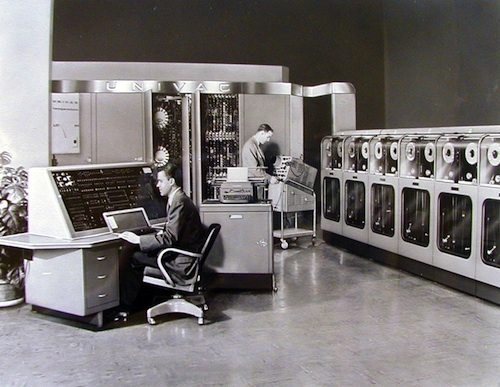
\includegraphics[width=0.7\textwidth]{images/computer}
      \caption{Quelle: Wikipedia}
\end{figure}
\end{block}

 \end{frame}

\begin{frame}
    \frametitle{Angewandte Mathematik}
\framesubtitle{Fehleranalyse}
\begin{figure}[H]
      \centering
    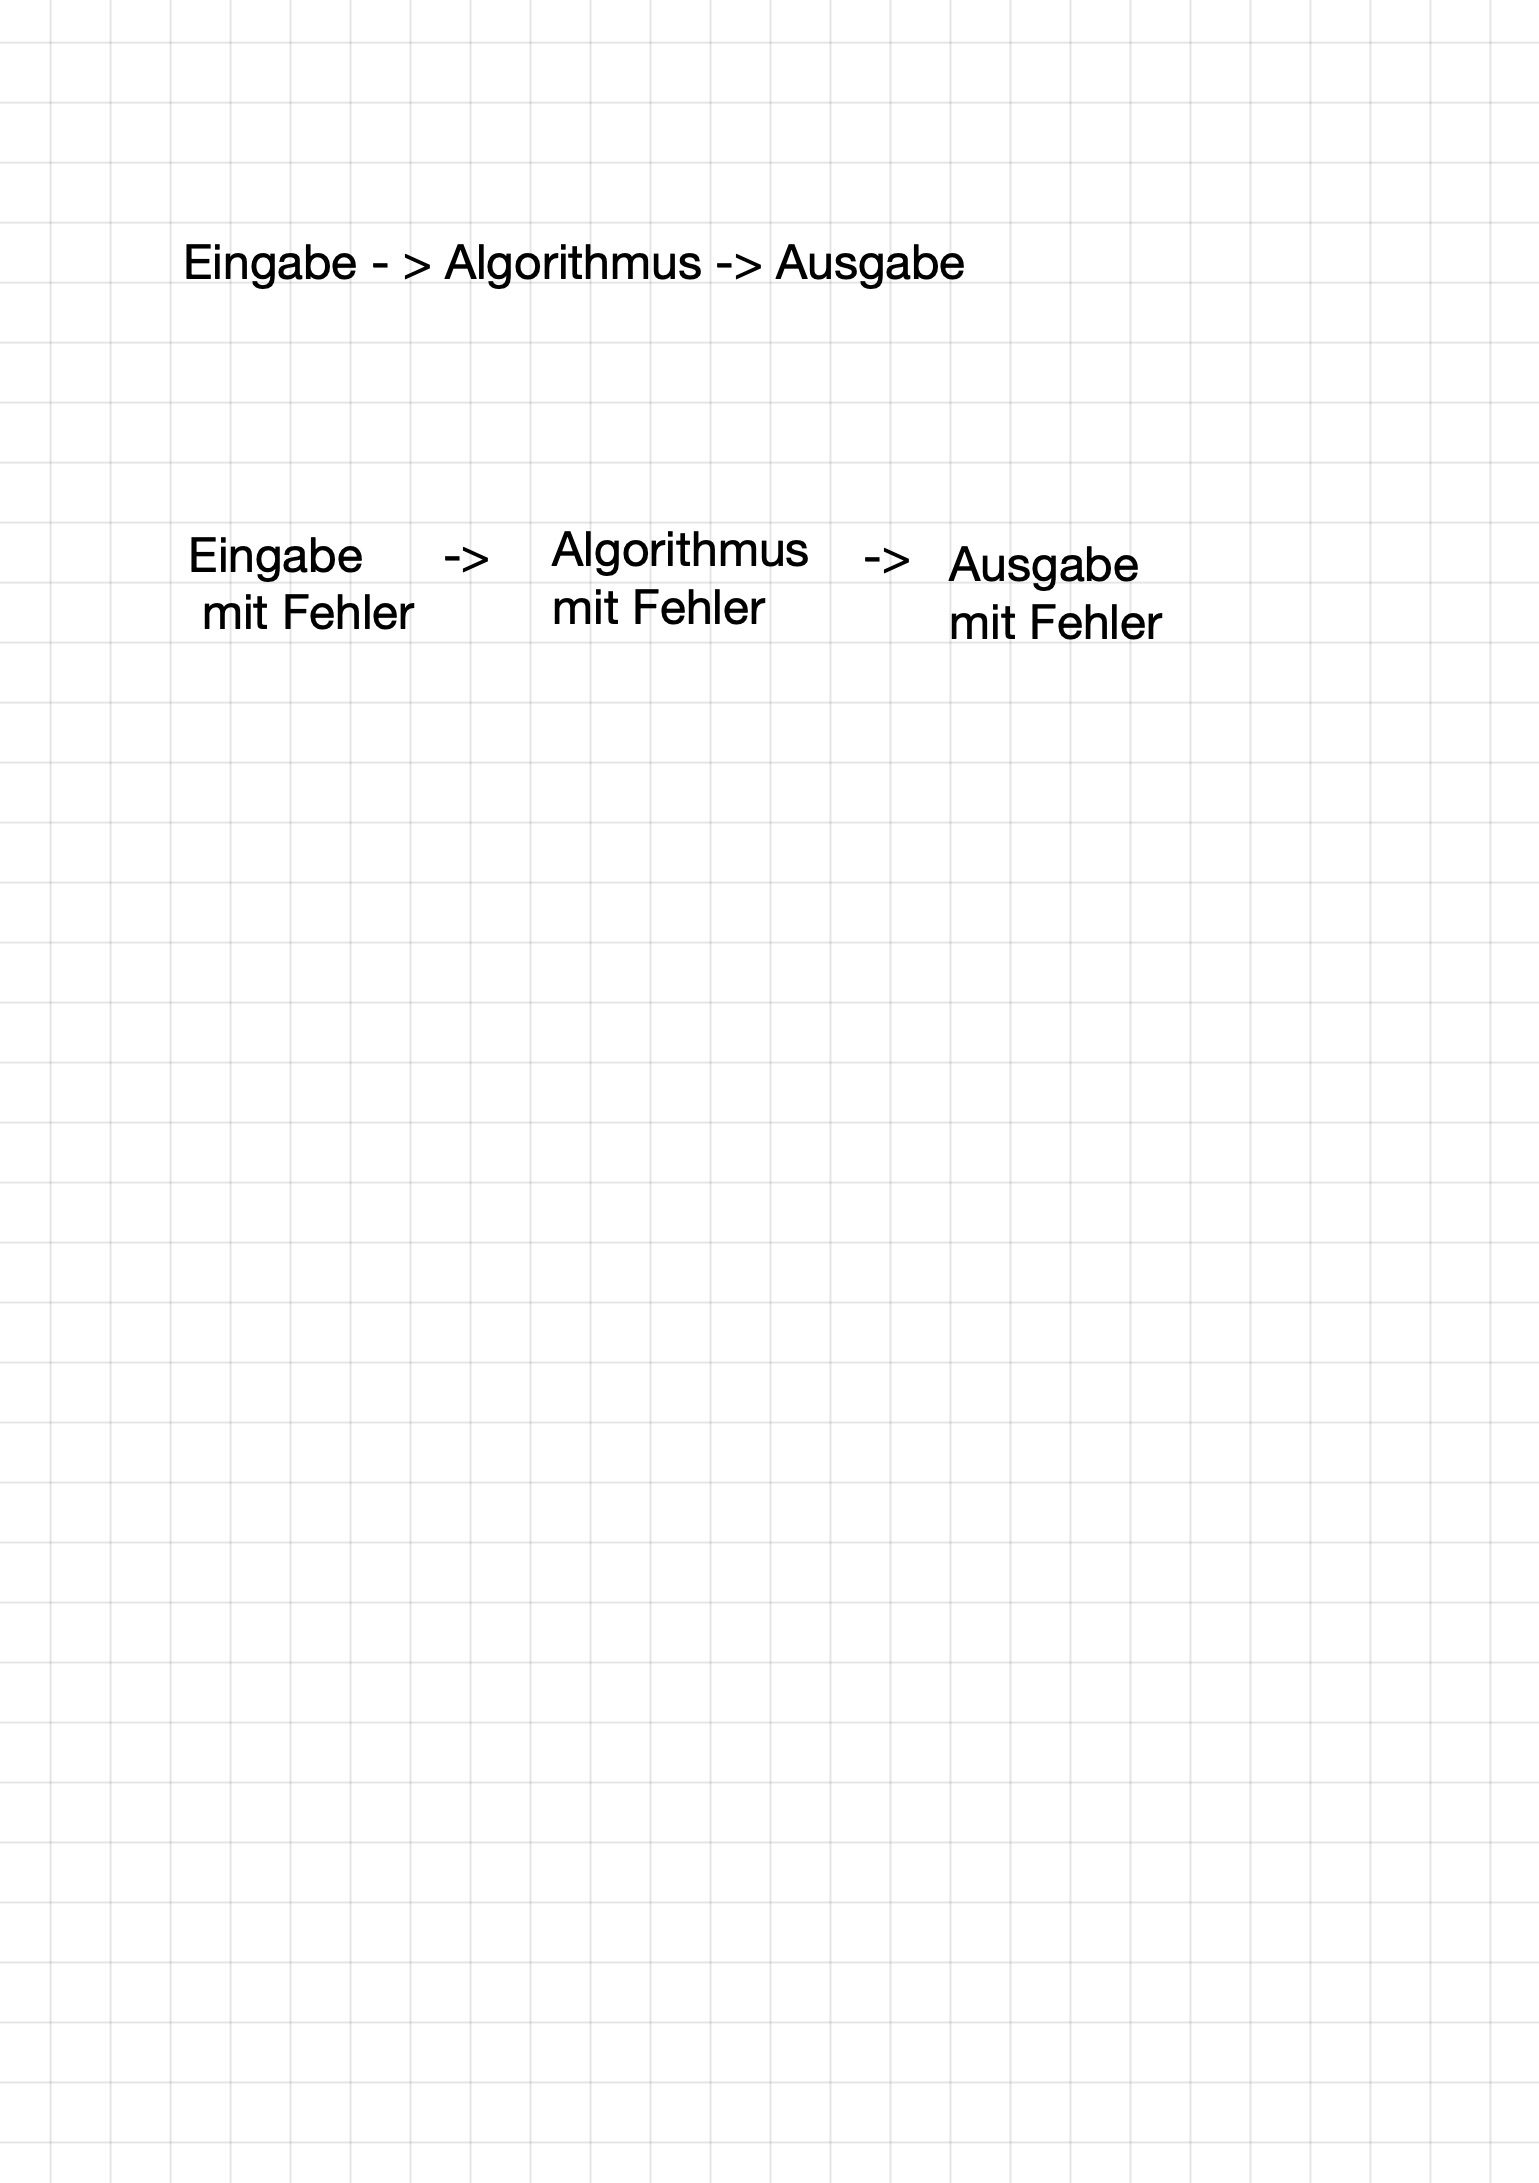
\includegraphics[width=0.7\textwidth]{images/fehler}\end{figure}
 \end{frame}


\begin{frame}
    \frametitle{Angewandte Mathematik}
\framesubtitle{Fehleranalyse}
    \begin{block}{Gleitkommazahl}
Eine Gleitkommazahl ist eine Zahl $z$ der Form
\begin{align*}
z = a d^e \\
a = (\pm) \sum_{i=1}^ld^{-l} \\
e \in \{e_{min}, \cdots , e_{max}  \} \subset \mathbb{Z}
\end{align*}
Auf einem Computer ist $d=2$.
\end{block}

    \begin{block}{Gleitkommazahl}
Beispiel mit  $d= 10$ 
\begin{align*}
0.314156 \cdot 10^1
\end{align*}
\end{block}

 \end{frame}



\begin{frame}
    \frametitle{Angewandte Mathematik}
\framesubtitle{Fehleranalyse}
    \begin{block}{Gleitkommazahl}
Ist x eine reelle Zahl so gibt es eine  Gleitkommazahl $fl(x)$ mit
\begin{align*}
\frac{|x-fl(x)| }{|x|} \leq eps := d^{1-l}/2
\end{align*}
\end{block}

 \end{frame}



\begin{frame}
    \frametitle{Angewandte Mathematik}
\framesubtitle{Fehleranalyse}
    \begin{block}{Gleitkommazahl}
Für eine exakte Operation $\circ \in \{+,-, \cdot, : \}$ gilt für die entsprechende Ausführung $\hat{\circ}$ auf einem Computer
\begin{align*}
a \hat{\circ}  b = (a \circ b) (1  + \epsilon) , \ \epsilon \leq eps 
\end{align*}
\end{block}
 \end{frame}


\begin{frame}
    \frametitle{Angewandte Mathematik}
\framesubtitle{Fehleranalyse}
    \begin{block}{Konditionszahl}
 Die Kondition beschreibt  die Abhängigkeit der Lösung eines Problems von der Störung der Eingangsdaten.  Die Konditionszahl stellt ein Maß für diese Abhängigkeit dar. Sie beschreibt das Verhältnis von  $E:= \{\widetilde{x} \; | \; ||\widetilde{x} -x || \leq eps ||x|| \}$ zu $R: = \{f(\widetilde{x}) \; | \; \widetilde{x} \in E \}$.
\end{block}
\begin{figure}[H]
      \centering
    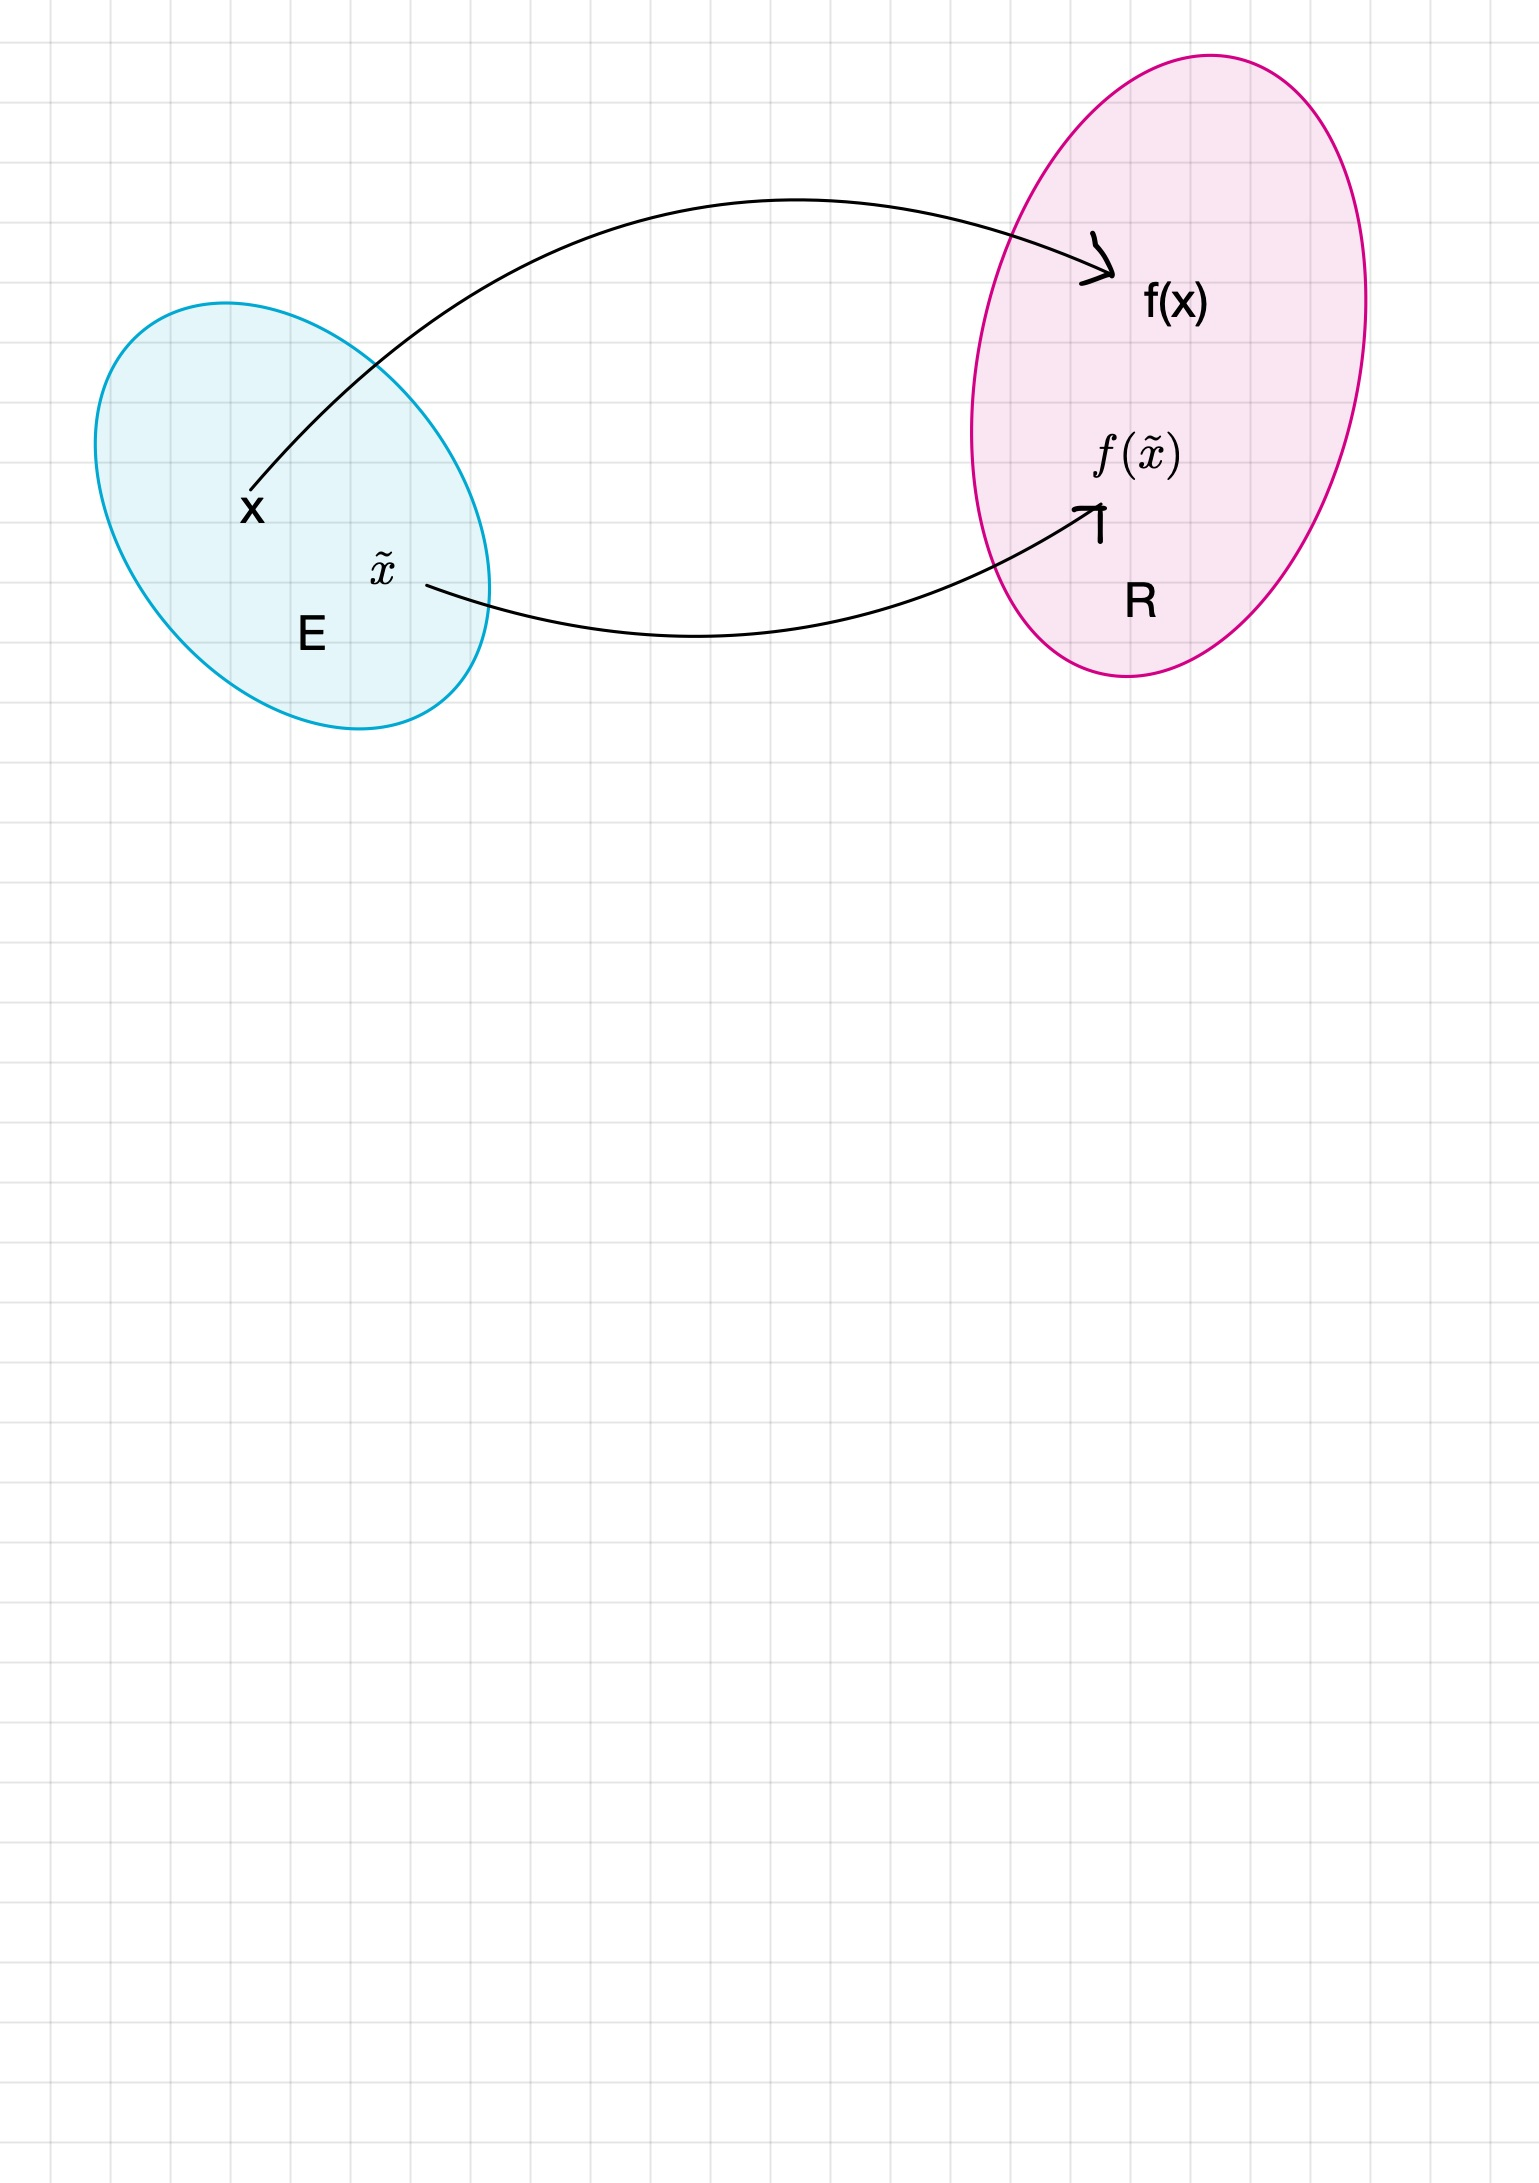
\includegraphics[width=0.8\textwidth]{images/kondition}
      \caption{}
\end{figure}

 \end{frame}



\begin{frame}
    \frametitle{Angewandte Mathematik}
\framesubtitle{Fehleranalyse}
    \begin{block}{Kondition eines Problems}
Die absolute Konditionierung eines Problems $(f,x)$ ist die Kleinste Zahl $\kappa_{abs}$ mit 
\begin{align*}
|| f(x) - f(\widetilde{x}) || \leq \kappa_{abs} || x - \widetilde{x} || , \;  \widetilde{x} \to x
\end{align*}
\end{block}

    \begin{block}{Kondition eines Problems}
Die relative  Konditionierung eines Problems $(f,x)$ ist die Kleinste Zahl $\kappa_{rel}$ mit 
\begin{align*}
\frac{|| f(x) - f(\widetilde{x}) ||}{||f(x) || } \leq \kappa_{rel} \frac{|| x - \widetilde{x} ||}{||x||} , \; \widetilde{x} \to x
\end{align*}
\end{block}

 \end{frame}


\begin{frame}
    \frametitle{Angewandte Mathematik}
\framesubtitle{Fehleranalyse}
    \begin{block}{Kondition eines Problems}
Momentan können wir noch keine Konditionszahlen berechnen. Wir werden später lernen, wie wir sie in vielen Fällen abschätzen können.
\end{block}
 \end{frame}




\begin{frame}
    \frametitle{Angewandte Mathematik}
\framesubtitle{Fehleranalyse}
    \begin{block}{Stabilität}
\end{block}
\begin{figure}[H]
      \centering
    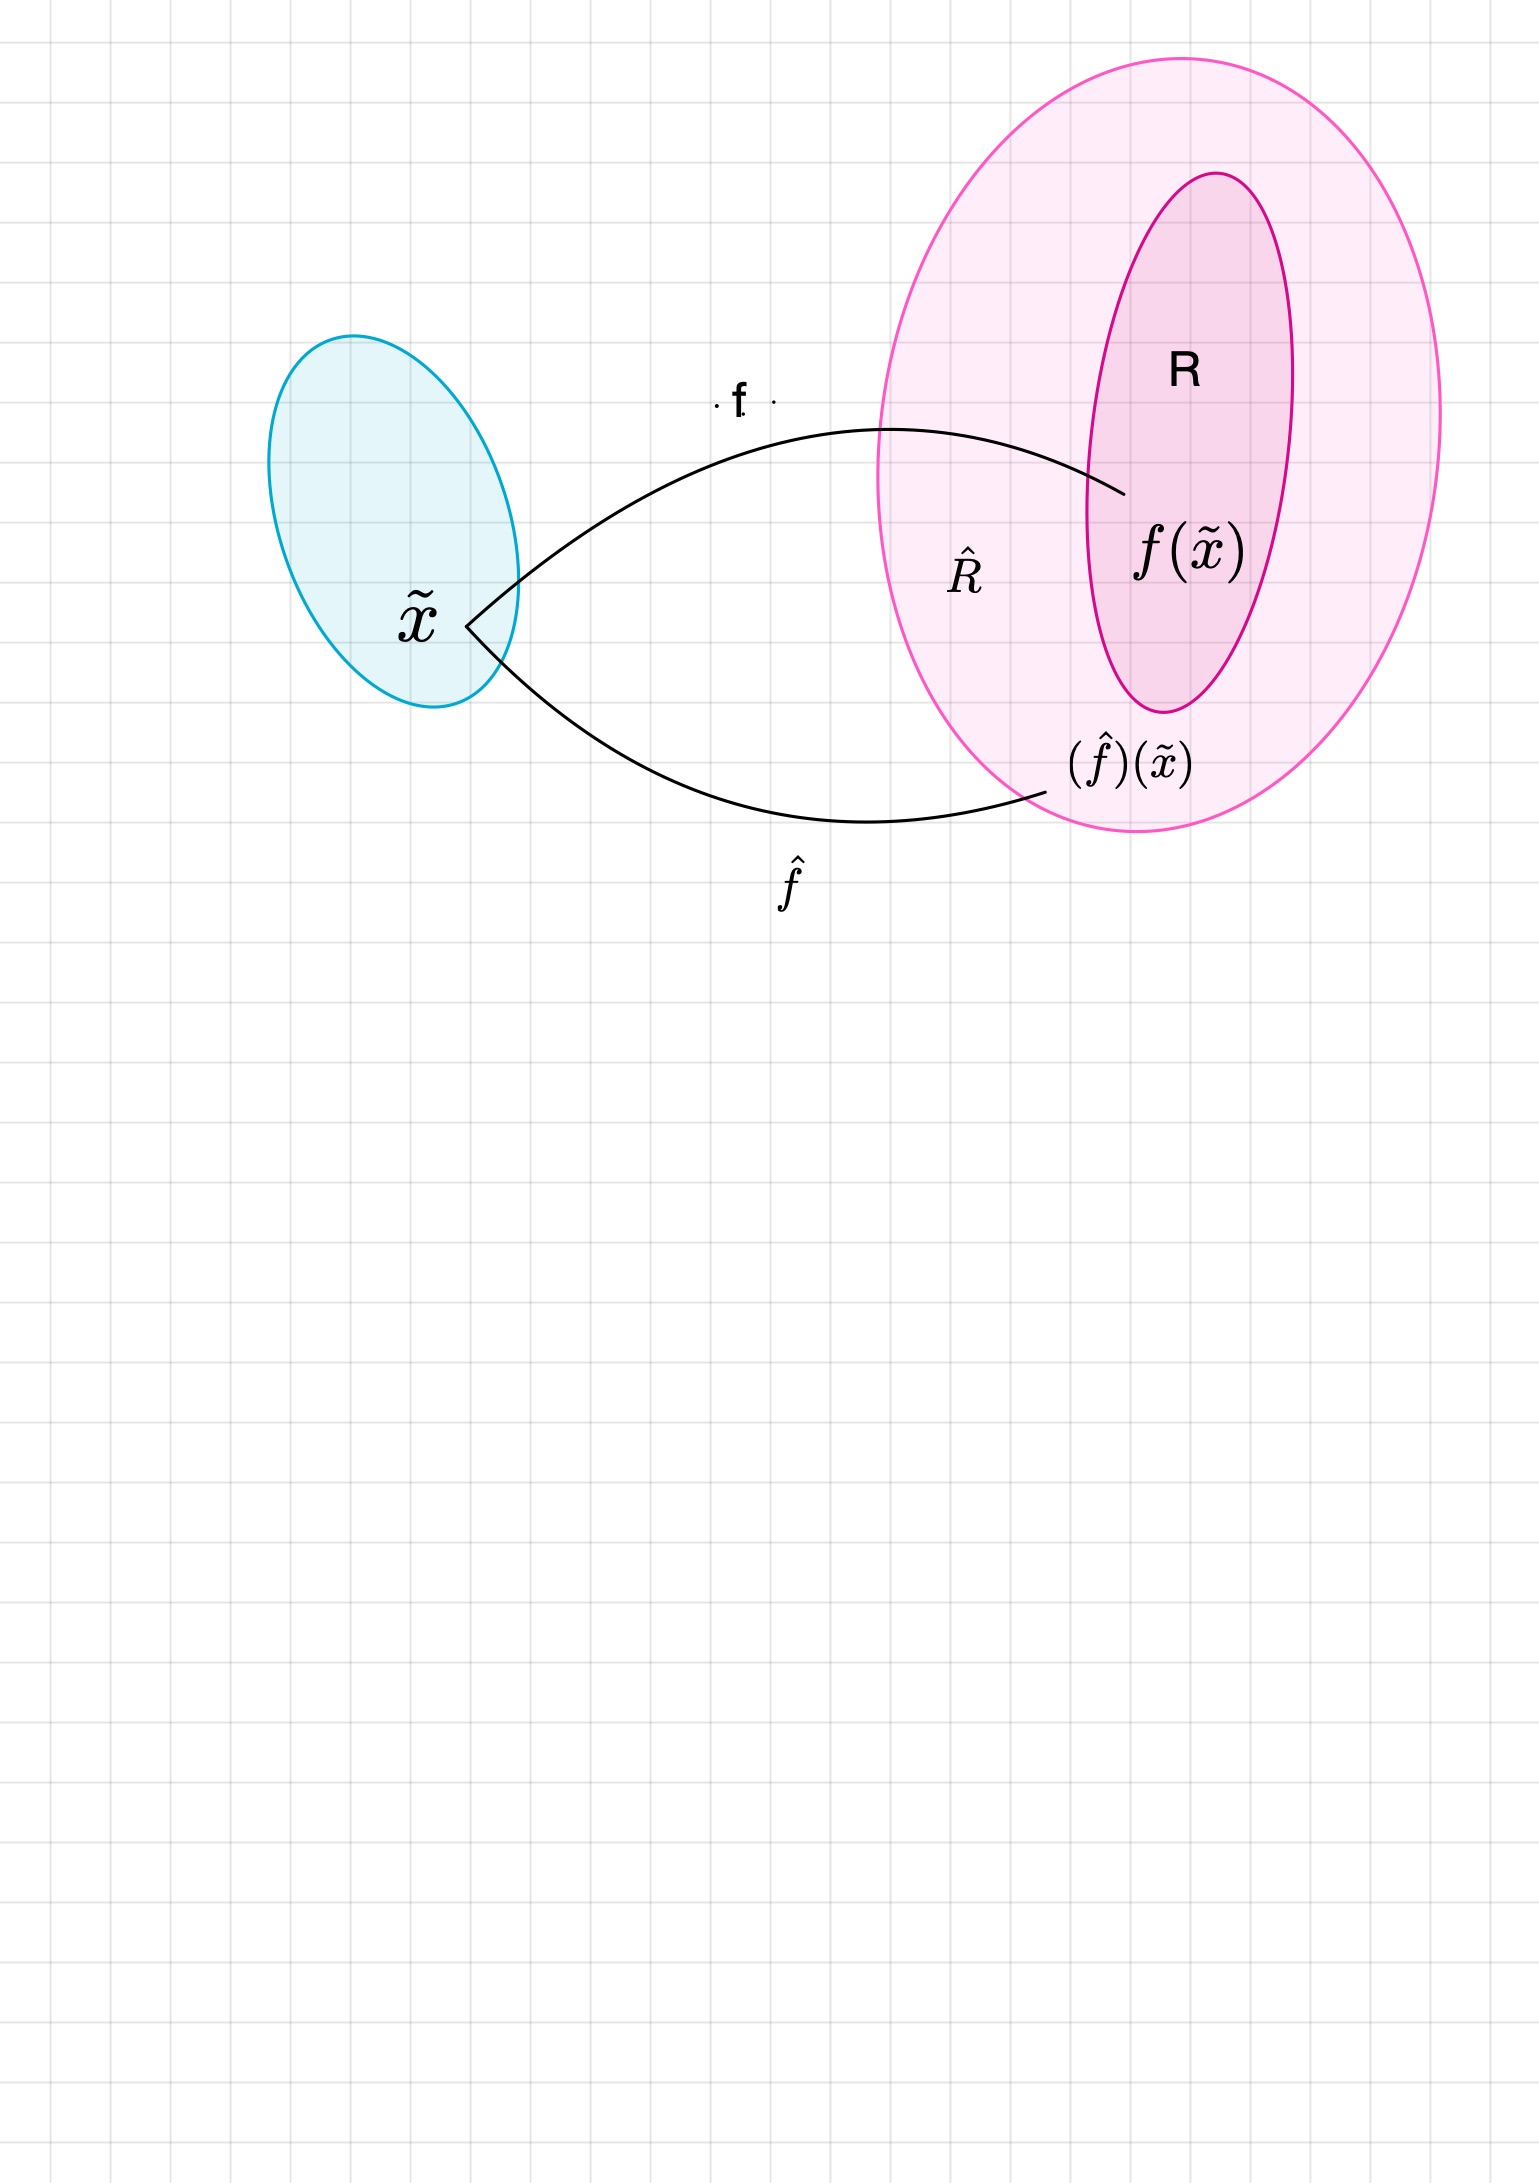
\includegraphics[width=0.8\textwidth]{images/stabilitaet}
      \caption{}
\end{figure}
 \end{frame}



\begin{frame}
    \frametitle{Angewandte Mathematik}
\framesubtitle{Fehleranalyse}
    \begin{block}{Stabilität}
Für eine Gleikommarealisierung $\hat{f}$ eines Algorithmus zur Lösung des Problems $(f,x)$ mit relativer Konditionszahl $\kappa_rel$ ist der Stabilitätsindikator definiert als die kleinste Zahl $\sigma \geq 0$ mit 
\begin{align*}
\frac{|| \hat{f}(\widetilde{x}) - f(\widetilde{x}) ||}{||f(\widetilde{x}) || } \leq \sigma  \kappa_{rel} eps , \; eps \to 0
\end{align*}
für alle $\widetilde{x} \in E$
\end{block}
    \begin{block}{Stabilität eines Algorithmus}
Der Algorithmus $\hat{f}$ heisst stabil, wenn $\sigma$ kleiner ist als die Anzahl der hintereinander ausgeführten Elementaroperationen. 
\end{block}
 \end{frame}

\end{document}

